%----------------------------------------------------------------------------------------
%	CONSTANTS
%----------------------------------------------------------------------------------------

\newcommand{\hmwkTitle}{Report\ \#4}					% Assignment title
\newcommand{\hmwkClass}{Communication Networks}			% Course name
\newcommand{\hmwkClassTime}{}							% Workshop time
\newcommand{\hmwkClassInstructor}{}						% Tutor name
\newcommand{\hmwkAuthorName}{Ang LEE}					% Student name

\newcommand{\hmwkGraphicsPath}{img/}					% Graphics path
\newcommand{\hmwkCodePath}{code/}						% Code path

%----------------------------------------------------------------------------------------
%	TEMPLATE
%----------------------------------------------------------------------------------------

\documentclass{article}

\usepackage{fancyhdr}	% Required for custom headers
\usepackage{lastpage}	% Required to determine the last page for the footer
\usepackage{extramarks} % Required for headers and footers
\usepackage{graphicx}	% Required to insert images
\graphicspath{\hmwkGraphicsPath}
\usepackage{lipsum} 	% Used for inserting dummy 'Lorem ipsum' text into the template

\usepackage{float}
\usepackage{epstopdf}	% Required to insert .eps images
\usepackage{amssymb}
\usepackage{amsmath}
\usepackage[hidelinks]{hyperref}
\usepackage{tabu}		% Required to insert table of certain width

% Python syntax highlighting
\usepackage{color}		% Required to define colors
\definecolor{commentColor}{RGB}{153,153,153}
\definecolor{stringColor}{RGB}{37,170,33}
\usepackage{listings}
\lstset{
	inputpath=\hmwkCodePath,
	language=Python,
	basicstyle=\footnotesize\codefont,
	keywordstyle=\color{blue},
	stringstyle=\color{stringColor},
	commentstyle=\usefont{T1}{pcr}{m}{n}\color{commentColor},
	breaklines=true,
	showstringspaces=false,
	numbers=left,
	numberstyle=\scriptsize,
	firstnumber=1,
	numberfirstline=true,
	stepnumber=5,
	frame=leftline
}

\usepackage{fontspec}
\newfontfamily\codefont{Lucida_Console.ttf}
\setsansfont[BoldFont=Lucida_Grande_Bold.ttf]{Lucida_Grande.ttf}

% change \textbf textbf
\definecolor{bfcolor}{RGB}{221,75,57}
\DeclareTextFontCommand{\textbf}{\bfseries\color{bfcolor}}

% change \texttt color
\definecolor{ttcolor}{RGB}{0,103,179}
\DeclareTextFontCommand{\texttt}{\ttfamily\color{ttcolor}}

% change headings color
\usepackage{sectsty}
\definecolor{sectioncolor}{RGB}{0,102,33}
\sectionfont{\color{sectioncolor}\sffamily}
\definecolor{subsectioncolor}{RGB}{26,131,171}
\subsectionfont{\color{subsectioncolor}\sffamily}
\definecolor{subsubsectioncolor}{RGB}{0,51,102}
\subsubsectionfont{\color{subsubsectioncolor}\sffamily}

% Margins
\topmargin=-0.45in
\evensidemargin=0in
\oddsidemargin=0in
\textwidth=6.5in
\textheight=9.0in
\headsep=0.25in

\linespread{1.1}		% Line spacing

% Set up the header and footer
\pagestyle{fancy}
\lhead{\hmwkTitle} % Header Left 
\chead{\hmwkAuthorName} % Header Center
\rhead{\hmwkClass} % Header Right
\lfoot{\url{https://github.com/leeang/Communication-Networks}} % Footer Left
\cfoot{} % Footer Center
\rfoot{Page\ \thepage\ of\ \pageref{LastPage}} % Footer Right
\renewcommand\headrulewidth{0.4pt} % Size of the header rule
\renewcommand\footrulewidth{0.4pt} % Size of the footer rule

\setlength\parindent{0pt} % Removes all indentation from paragraphs

%----------------------------------------------------------------------------------------
%	Problem and Section
%----------------------------------------------------------------------------------------

\newenvironment{homeworkProblem}[1]{
	\section*{#1}
	}{
}
\newenvironment{homeworkSection}[1]{
	\subsection*{#1}
	}{
}
\newcommand{\problemAnswer}[1]{
	\noindent\framebox[\columnwidth][c]{
		\begin{minipage}{0.98\columnwidth}
			#1
		\end{minipage}
	}
}

%----------------------------------------------------------------------------------------
%	Document
%----------------------------------------------------------------------------------------

\begin{document}

\newpage

%----------------------------------------------------------------------------------------
%	Section 1
%----------------------------------------------------------------------------------------

\begin{homeworkProblem}{Question 1.1}
Briefly explain what GET and POST mean in HTTP? What are the other request methods in HTTP version 1.1?\\

The \texttt{GET} method means retrieve whatever information (in the form of an entity) is identified by the Request-URI. If the Request-URI refers to a data-producing process, it is the produced data which shall be returned as the entity in the response and not the source text of the process, unless that text happens to be the output of the process.\\

The \texttt{POST} method is used to request that the origin server accept the entity enclosed in the request as a new subordinate of the resource identified by the Request-URI in the Request-Line.\\

\texttt{OPTIONS}, \texttt{HEAD}, \texttt{PUT}, \texttt{DELETE}, \texttt{TRACE} and \texttt{CONNECT}.\\

Reference: \url{http://www.w3.org/Protocols/rfc2616/rfc2616-sec9.html}
\end{homeworkProblem}

%--------------------------------------------

\begin{homeworkProblem}{Question 1.2}
Describe what the program \texttt{simple\_webserver.py} does couple of sentences.

\begin{enumerate}
\item main function establishes an HTTP server at localhost:80 listening at the HTTP socket
\item \texttt{do\_GET()} and \texttt{do\_POST()} determines how to response \texttt{GET()} and \texttt{POST()} request method respectively
\end{enumerate}
\end{homeworkProblem}

%--------------------------------------------

\begin{homeworkProblem}{Question 1.3}
What does the code 200 in \texttt{self.send\_response(200)} in that program mean? Name another very commonly used HTTP response code and explain its meaning.\\

\textbf{200 OK}\\
The request has succeeded.\\

The information returned with the response is dependent on the method used in the request, for example:\\
\texttt{GET} an entity corresponding to the requested resource is sent in the response;\\
\texttt{POST} an entity describing or containing the result of the action.\\

\textbf{404 Not Found}\\
The server has not found anything matching the Request-URI. No indication is given of whether the condition is temporary or permanent. This status code is commonly used when the server does not wish to reveal exactly why the request has been refused, or when no other response is applicable.\\

Reference: \url{http://www.w3.org/Protocols/rfc2616/rfc2616-sec10.html}
\end{homeworkProblem}

%--------------------------------------------

\begin{homeworkProblem}{Question 1.4}
Based on your observations in Step 1.2, explain briefly what the function \texttt{do\_Get()} in \texttt{simple\_webserver.py} does.\\

\texttt{info\_messgage()} function analyses client values and server values as well as headers.\\

\textbf{CLIENT VALUES}\\
client address, command, path, real path, query, request version\\

\textbf{SERVER VALUES}\\
server version, sys version (i.e. python version), protocol version\\

\textbf{HEADERS}\\
accept, accept-encoding, accept-language, cache-control, connection, host, upgrade-insecure-requests and user-agent\\

\texttt{do\_GET()} function primarily generates a simple HTML and displays the data retrieved by \texttt{info\_messgage()}.
\end{homeworkProblem}

%--------------------------------------------

\begin{homeworkProblem}{Question 1.5}
Based on your observations in Step 1.3, explain briefly what the function \texttt{do\_Post()} in \texttt{simple\_webserver.py} does.\\

\texttt{do\_POST()} displays client address, user-agent, path (`/post\_form' in this case) and the form data `FirstName', `LastName' and their values (`Mickey' and `Mouse' by default) submitted in \texttt{formexample.html}
\end{homeworkProblem}

%--------------------------------------------

\begin{homeworkProblem}{Question 1.6}
Comment on the differences between the client we wrote and a browser, based on your observations. Which one is suited for which role(s)?\\

\textbf{CLIENT VALUES}\\
client address, path, real path and query are apparently different.\\

\textbf{SERVER VALUES}\\
the same.\\

\textbf{HEADERS}\\
accept, accept-encoding and user-agent are different. Request generated by client does not have `accept-language' and `upgrade-insecure-requests' fields.\\

In my opinion, modern browsers such as Chrome, Firefox and Microsoft Edge are rich and sophisticated clients specialized in web pages demonstration and human computer interaction. For example, the layout engine built in web browser renders HTML and CSS to an interactive document and JavaScript interpreter enables browser-end programming. Images, audios and videos are also supported by browsers.\\

However, clients are thin, light-weight and customized to realize certain logic. Unlike browsers, applications in clients can also invoke underlying protocols not limited to HTTP and HTTPS.\\

As a result, clients are suited for machines and browsers are suited for humans.
\end{homeworkProblem}

%----------------------------------------------------------------------------------------
%	Section 2
%----------------------------------------------------------------------------------------

\begin{homeworkProblem}{Question 2.1}
Demand management falls under the umbrella of smart grid. Why does the grid become smart when there is demand response? What makes the legacy grid not so smart and which new feature(s) changes this?\\

The grid becomes smart when there is demand response because electricity users (e.g. households, business, industry) can adjust their power load when the total demand in the whole grid changes. The grid benefits from this mechanism by reducing surges and smoothing fluctuations in electricity demand.\\

Big industrial sites have made agreements with power companies to reduce their demand at peak times. However, this service is infeasible to be expanded to individual clients due to the high cost of human intervention. Hence, \textbf{demand management automation} is necessary in smart grid.
\end{homeworkProblem}

%--------------------------------------------

\begin{homeworkProblem}{Question 2.2}
Discuss very briefly the similarities and differences between the transitions from the old telephony system to Internet and the legacy power network to the modern power grid.\\

Old telephony system commonly employs analog signal to transmit voice over copper loops with limited bandwidth and susceptible to distortion. Modern Internet has larger capacity and is born with error detection and correction mechanism. In fact, the old telephony system is fiercely challenged by Voice over IP technology. In spite of the advent of the smart gird, the main task of grid is to carry electricity. Hence, I think the legacy power grid will be attributed new feature such as demand management automation. Perhaps in the future, the smart grid will be a amalgamation of legacy power grid and Internet. For example, broadband over power lines is a method of power line communication that allows relatively high-speed digital data transmission over the public electric power distribution wiring.
\end{homeworkProblem}

%----------------------------------------------------------------------------------------
%	Section 3
%----------------------------------------------------------------------------------------

\begin{homeworkProblem}{Question 3.1}
Provide a working copy of the program you write according to the guidelines for full credit. Note that this is an open-ended question. Feel free to use your creativity!

\begin{homeworkSection}{Price simulation}
We want to simulate price change over 24h based on `avg\_pricelist' returned by \texttt{import\_pricedata()} function. Noticing that data in \texttt{GRAPH\_5VIC1.csv} starts from 12/07/2014 12:35, we decide to \textbf{circularly shift} the python list in order to match price and the real time.\\

For instance, the 30min average price out of six points (12/07/2014 12:35, 12:40, 12:45, 12:50, 12:55) is used to simulate the real price in the time period from 12:30:01 to 13:00:00, the 30min average price out of six points (13/07/2014 0:05, 0:10, 0:15, 0:20, 0:25) is used to simulate the real price in the time period from 00:00:01 to 00:30:00. More examples are available in the following table.
\begin{table}[!hbp]
\centering
\begin{tabu} to 0.8\textwidth {X[c] X[l] X[l]}
avg\_pricelist index &time in csv &real time\\
0  & 2014-07-12 12:35$\sim$13:00 & 12:30:01$\sim$13:00:00 \\
1  & 2014-07-12 13:05$\sim$13:30 & 13:00:01$\sim$13:30:00 \\
2  & 2014-07-12 13:35$\sim$14:00 & 13:30:01$\sim$14:00:00 \\
$\cdots$ &$\cdots$ &$\cdots$\\
22 & 07-12 23:35$\sim$07-13 0:00  & 23:30:01$\sim$00:00:00 \\
23 & 2014-07-13 0:05$\sim$0:30   & 00:00:01$\sim$00:30:00 \\
24 & 2014-07-13 0:35$\sim$1:00   & 00:30:01$\sim$01:00:00 \\
$\cdots$ &$\cdots$ &$\cdots$\\
46 & 2014-07-13 11:35$\sim$12:00 & 11:30:01$\sim$12:00:00
\end{tabu}
\end{table}

This arithmetic is implemented by \texttt{get\_price()} function in \texttt{webserver.py} and \texttt{import\_pricedata()} function in \texttt{pricetempreader.py}.
\end{homeworkSection}

%--------------------------------------------

\begin{homeworkSection}{Temperature measurement simulation}

We want to simulate temperature change over 24h based on `temperature' returned by \texttt{import\_tempdata()} function. Noticing that data in \texttt{IDV60901.94868.json} was sorted by their time in descending order (latest entries listed first), we modify \texttt{import\_tempdata()} function slightly, i.e. select data with `sort\_order' from 28 to 75 and output in reverse order.
\begin{table}[!hbp]
\centering
\begin{tabu} to 0.8\textwidth {X[c] X[l] X[l]}
sort\_order &local time in json &real time\\
75 & 2014-07-12 00:00:00 & 00:00:00$\sim$00:29:59 \\
74 & 2014-07-12 00:30:00 & 00:30:00$\sim$00:59:59 \\
$\cdots$ &$\cdots$ &$\cdots$\\
29 & 2014-07-12 23:00:00 & 23:00:00$\sim$23:29:59 \\
28 & 2014-07-12 23:30:00 & 23:30:00$\sim$23:59:59
\end{tabu}
\end{table}

This arithmetic is implemented by \texttt{get\_temperature()} function in \texttt{webclient.py} and \texttt{import\_tempdata()} function in \texttt{pricetempreader.py}.
\end{homeworkSection}

%--------------------------------------------

\begin{homeworkSection}{Simulation result}
\begin{figure}[H]
\begin{minipage}[t]{0.5\linewidth}
\centering
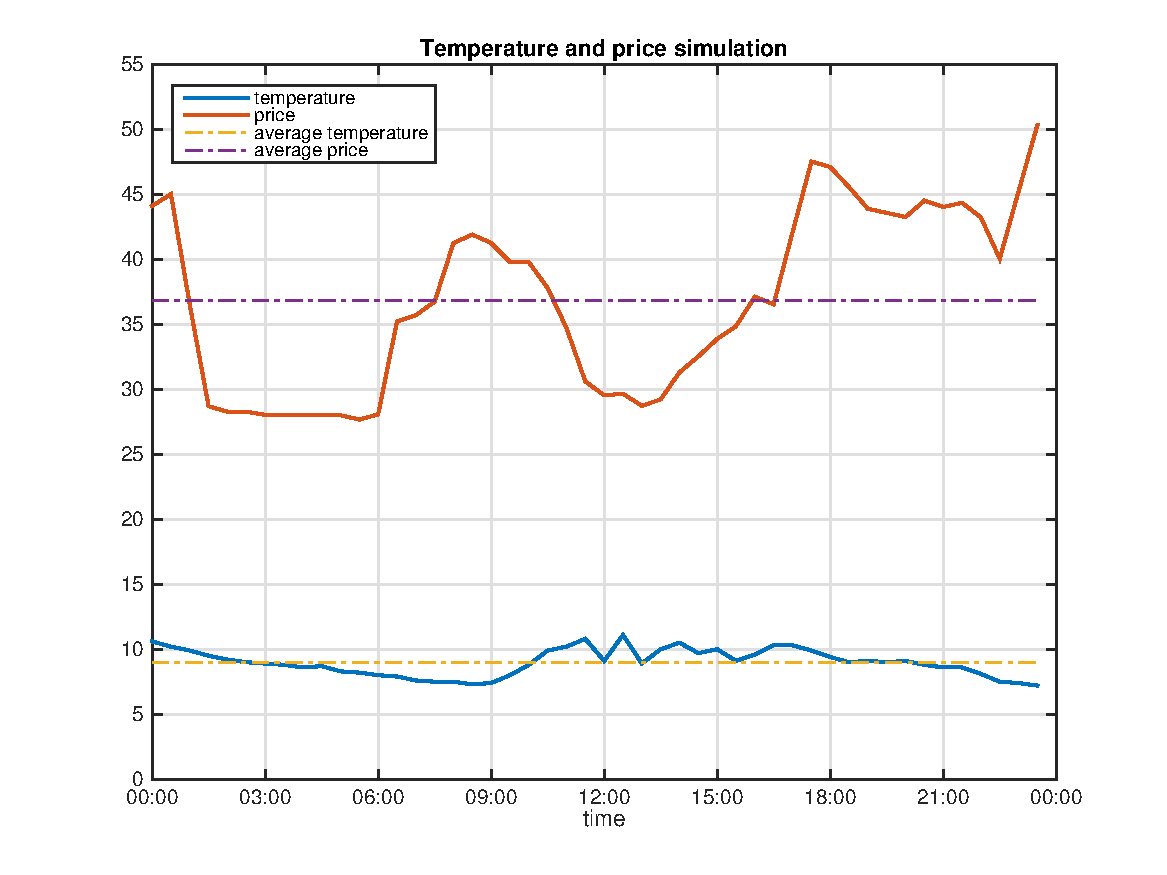
\includegraphics[width=\linewidth]{temperature_price}
\caption{Price and temperature over 24h}
\label{temperature_price}
\end{minipage}
\begin{minipage}[t]{0.5\linewidth}
\centering
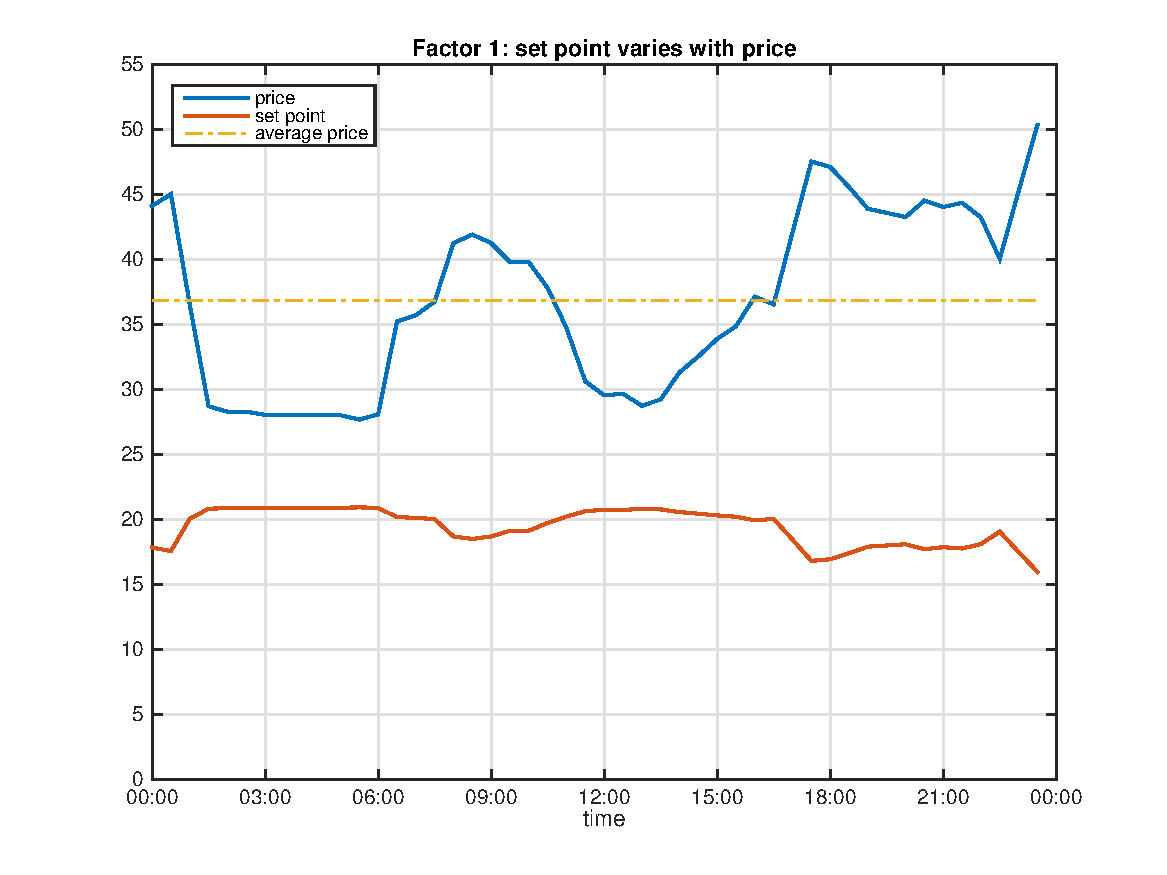
\includegraphics[width=\linewidth]{setpoint_price}
\caption{Set point varies with price}
\label{setpoint_price}
\end{minipage}
\end{figure}
\end{homeworkSection}

%--------------------------------------------

\begin{homeworkSection}{Set point decision strategy}
\subsubsection*{Outside temperature influence}
As can be clearly seen in Figure \ref{temperature_price}, temperature fluctuates around 8.98 degrees centigrade. This result is easy to understand, because 12th of July in Melbourne is during winter. Room temperature of 20 degrees is most comfortable for human, hence the house needs heating. The outside temperature will not be taken in to consideration when deciding set point.

\subsubsection*{Factor 1: price}
In order to save total expanse, we decide to tune down the set point when price is higher than the average price (AU\$ 36.87) and slightly turn it up and try to store some thermal energy when the price is low.
\begin{equation}
\text{set point} =
\begin{cases}
20 - 0.3 \times (\text{price} - \text{average price}) & \text{price} > \text{average price}\\
20 + 0.1 \times (\text{average price} - \text{price}) & \text{price} < \text{average price}
\end{cases}
\end{equation}
How price impacts on set point is shown in in Figure \ref{setpoint_price}.

\subsubsection*{Factor 2: daily routine}
It is believed that most people are sleeping in bed from 00:00 to 06:00. It is not necessary to keep the room warm during this period. We decide to gradually cool down and then warm up the house during these 6 hours. How daily routine impacts on set point is shown in in Figure \ref{setpoint_time}. Sharp transition is avoided.

\begin{figure}[H]
\begin{minipage}[t]{0.5\linewidth}
\centering
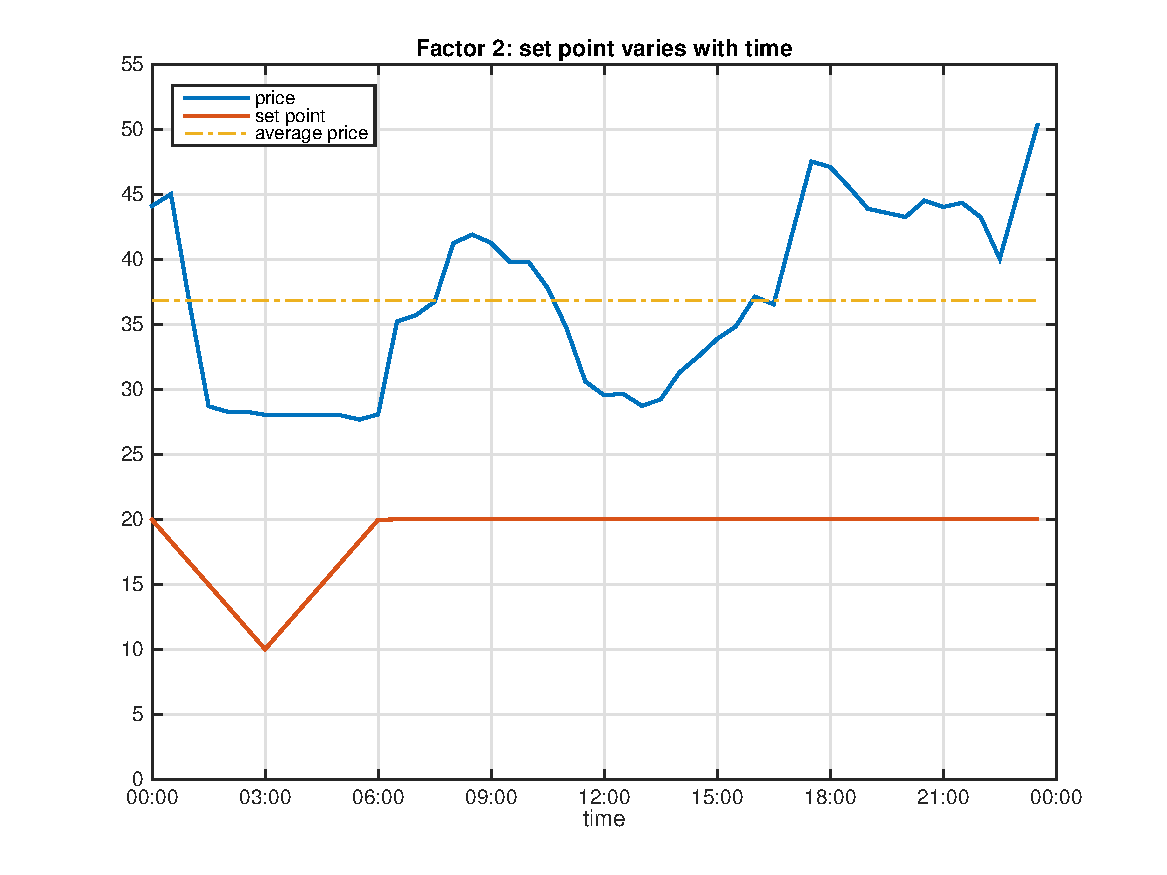
\includegraphics[width=\linewidth]{setpoint_time}
\caption{Set point varies with price}
\label{setpoint_time}
\end{minipage}
\begin{minipage}[t]{0.5\linewidth}
\centering
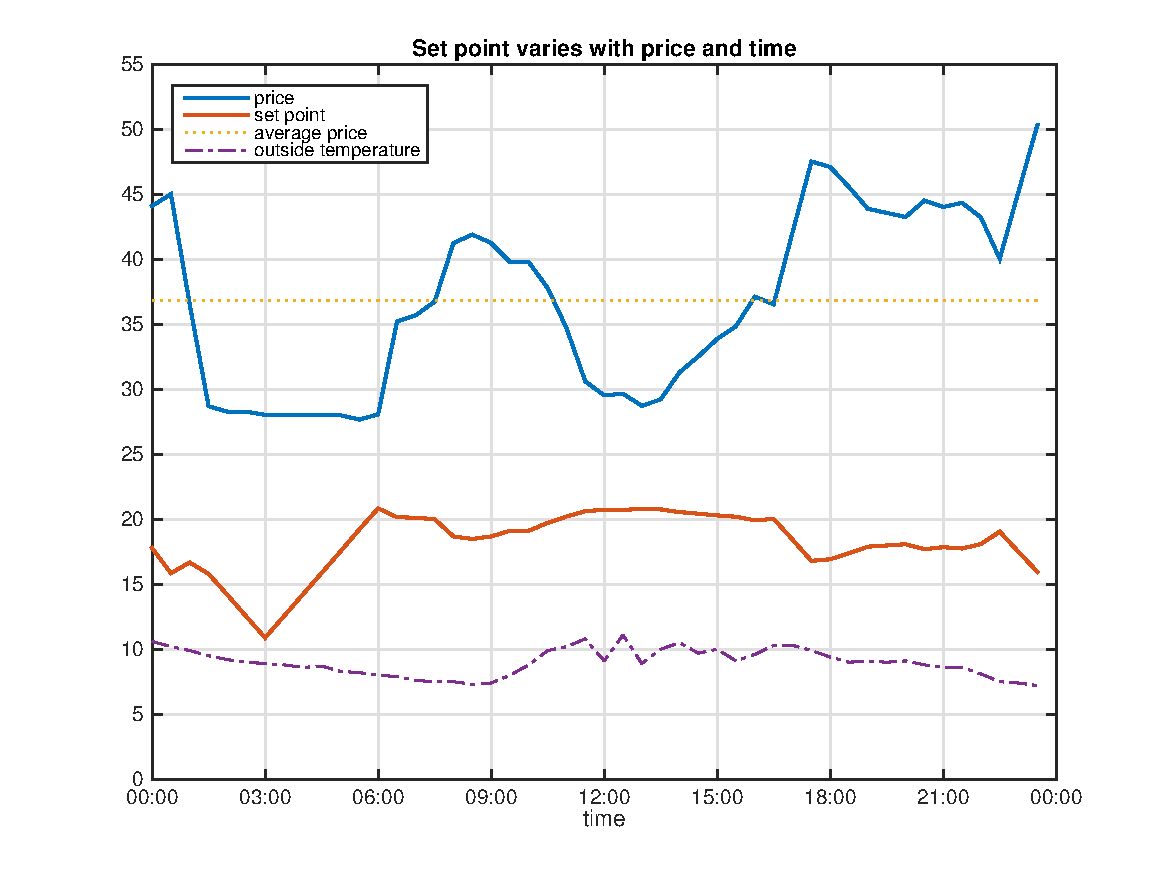
\includegraphics[width=\linewidth]{setpoint_price_time}
\caption{Set point varies with price and time}
\label{setpoint_price_time}
\end{minipage}
\end{figure}

\subsubsection*{Comprehensive influences}
Comprehensive influences are demonstrated in Figure \ref{setpoint_price_time}. Apparently, the set point changes from 10.88 to 20.83 degrees.

\end{homeworkSection}

%--------------------------------------------

\begin{homeworkSection}{Client information collection}

For demonstration purpose, we write client information such as \textbf{user name}, \textbf{temperature}, \textbf{set point} and current \textbf{timestamp} into a \texttt{.csv} file. In practical implementation, relational database management system (RDBMS) such as MySQL will be preferable.

\subsubsection*{\texttt{client-information.csv}}
user name, temperature, set point, timestamp
\lstinputlisting[language=tex]{client-information.csv}

\end{homeworkSection}

\end{homeworkProblem}

%----------------------------------------------------------------------------------------
%	Appendix
%----------------------------------------------------------------------------------------

\newpage
\begin{homeworkProblem}{Appendix}
\subsection*{\texttt{simulation\_and\_design.m}}
\lstinputlisting[language=matlab]{temperature_price.m}

\newpage
\subsection*{\texttt{webserver.py}}
\lstinputlisting{webserver.py}

\newpage
\subsection*{\texttt{webclient.py}}
\lstinputlisting{webclient.py}

\newpage
\subsection*{\texttt{pricetempreader.py}}
\lstinputlisting{pricetempreader.py}
\end{homeworkProblem}

%----------------------------------------------------------------------------------------

\end{document}
